% arara: pdflatex: { synctex: yes }
% arara: makeindex: { style: ctuthesis }
% arara: bibtex

% The class takes all the key=value arguments that \ctusetup does,
% and a couple more: draft and oneside
\documentclass[oneside]{ctuthesis}
\usepackage{siunitx}
\usepackage{nomencl}
\usepackage{setspace}
\usepackage{indentfirst}

%%%%%%%%%%%%%%%%%% insert images from other directory
\usepackage{graphicx}
\graphicspath{{./images/}}

%%%%%%%%%%%%%%%%%%%%%%%%%%%%%%%%%%%%%% this shit is here to break long url into more lines
\usepackage{url}
\makeatletter
\g@addto@macro{\UrlBreaks}{\UrlOrds}
%\makeatother

%%%%%%%%%%%%%%%%%%%%%%%%%%%%%%%%%%%%%% this shit is here to prevent breaking words on the edge of a line
\tolerance=1
\emergencystretch=\maxdimen
\hyphenpenalty=10000
\hbadness=10000


% to print code
\usepackage{listings}
\usepackage{color}
\definecolor{dkgreen}{rgb}{0,0.6,0}
\definecolor{gray}{rgb}{0.5,0.5,0.5}
\definecolor{mauve}{rgb}{0.58,0,0.82}
\lstset{frame=tb,
  language=Java,
  aboveskip=3mm,
  belowskip=3mm,
  showstringspaces=false,
  columns=flexible,
  basicstyle={\small\ttfamily},
  numbers=none, 
  % numberstyle=\tiny\color{gray},
  % keywordstyle=\color{blue},
  % commentstyle=\color{dkgreen},
  % stringstyle=\color{mauve},
  breaklines=true,
  breakatwhitespace=true,
  tabsize=3
}
% to display source code
\definecolor{mGreen}{rgb}{0,0.6,0}
\definecolor{mGray}{rgb}{0.5,0.5,0.5}
\definecolor{mPurple}{rgb}{0.58,0,0.82}
\definecolor{backgroundColour}{rgb}{0.95,0.95,0.92}
\lstdefinestyle{CStyle}{
    backgroundcolor=\color{backgroundColour},   
    commentstyle=\color{mGreen},
    keywordstyle=\color{magenta},
    numberstyle=\tiny\color{mGray},
    stringstyle=\color{mPurple},
    basicstyle=\footnotesize,
    breakatwhitespace=false,         
    breaklines=true,                 
    captionpos=b,                    
    keepspaces=true,                 
    numbers=left,                    
    numbersep=5pt,                  
    showspaces=false,                
    showstringspaces=false,
    showtabs=false,                  
    tabsize=2,
    language=C
}


%%%
% \usepackage{framed}
% \usepackage{hyperref}
% % \usepackage[czech]{babel}
% \usepackage[utf8]{inputenc}
% \usepackage[T1]{fontenc}

\usepackage{dirtree}        %directory tree visualisation
\usepackage{blindtext}
\parskip=12pt % adds vertical space between paragraphs

\usepackage{xcolor}
\definecolor{shadecolor}{RGB}{230,230,230}

% to print code
\usepackage{listings}
\usepackage{color}
%%%

\ctusetup{
%	preprint = \ctuverlog,```%%%%%%%%%%%%%%%%%%%%%%%%% toto je cislo na kazde strance dole ktere tam nema byt
%	mainlanguage = english,
%	titlelanguage = english,
	mainlanguage = czech,
	otherlanguages = {czech},
	title-czech = {Low power wireless sensor network},
	title-english = {Low power wireless sensor network},
	subtitle-czech = {},
	subtitle-english = {},
	faculty = F3,
	department-czech = {Katedra telekomunikační techniky},
	department-english = {Department of Telecommunications Engineering},
	author = {Tomáš Hyhlík},
	supervisor = {Ing. Bc. Marek Neruda, Ph.D},
	supervisor-address = {},
	supervisor-specialist = {Ing. Bc. Lukáš Vojtěch, Ph.D},
	fieldofstudy-english = {Electronics and Communications},
	subfieldofstudy-english = {Electronics},
	fieldofstudy-czech = {Elektronika a komunikace},
	subfieldofstudy-czech = {Elektronika},
	% keywords-czech = {sensor network},
	% keywords-english = {sensor network},
	day = 12,
	month = 10,
	year = 2019,
	specification-file = {zav_prace.pdf},
%	front-specification = true,
%	front-list-of-figures = false,
%	front-list-of-tables = false,
%	monochrome = true,
%	layout-short = true,
}

\ctuprocess

\addto\ctucaptionsczech{%
	\def\supervisorname{Vedoucí}%
	\def\subfieldofstudyname{Studijní program}%
}

\ctutemplateset{maketitle twocolumn default}{
	\begin{twocolumnfrontmatterpage}
		% \ctutemplate{twocolumn.thanks}
		% \ctutemplate{twocolumn.declaration}
		\ctutemplate{twocolumn.abstract.in.titlelanguage}
		\ctutemplate{twocolumn.abstract.in.secondlanguage}	
		\ctutemplate{twocolumn.tableofcontents}
		\ctutemplate{twocolumn.listoffigures}
	\end{twocolumnfrontmatterpage}
}

% Theorem declarations, this is the reasonable default, anybody can do what they wish.
% If you prefer theorems in italics rather than slanted, use \theoremstyle{plainit}
\theoremstyle{plain}
\newtheorem{theorem}{Theorem}[chapter]
\newtheorem{corollary}[theorem]{Corollary}
\newtheorem{lemma}[theorem]{Lemma}
\newtheorem{proposition}[theorem]{Proposition}

\theoremstyle{definition}
\newtheorem{definition}[theorem]{Definition}
\newtheorem{example}[theorem]{Example}
\newtheorem{conjecture}[theorem]{Conjecture}

\theoremstyle{note}
\newtheorem*{remark*}{Remark}
\newtheorem{remark}[theorem]{Remark}

\setlength{\parskip}{5ex plus 0.2ex minus 0.2ex}

% % Abstract in Czech
% \begin{abstract-czech}
% Účelem této práce je...

% \end{abstract-czech}

% % Abstract in English
% \begin{abstract-english}
% The purpose of this work is...
% \end{abstract-english}

% % Acknowledgements / Podekovani
% \begin{thanks}
% I would like to thank Supervisor Ing. Bc. Marek Neruda Ph.D and Supervisor-specialist Ing. Bc. Lukáš Vojtěch Ph.D for helping me with this project. Also I would like to thank IMA s.r.o. company, which helped me to get compatible cards to the HID Prox Point plus reader, which is used for the second system design.
% \end{thanks}


% % Declaration / Prohlaseni
% \begin{declaration}
% I declare that I have developed the presented work independently and that I have
% listed all information sources used in accordance with the Methodical Guidelines on
% Maintaining Ethical Principles During the Preparation of Higher Education Theses.

% In Prague, \ctufield{day}.~\monthinlanguage{title}~\ctufield{year}
% \end{declaration}

% Only for testing purposes
\listfiles
\usepackage[pagewise]{lineno}
\usepackage{lipsum,blindtext}
\usepackage{mathrsfs} % provides \mathscr used in the ridiculous examples

\newcommand{\abbrlabel}[1]{\makebox[3cm][l]{\textbf{#1}\ \dotfill}}
\newenvironment{abbreviations}{\begin{list}{}{\renewcommand{\makelabel}{\abbrlabel}}}{\end{list}}


%%%%%%%%%%%%%%%%%%%%%%%%%%%%%%%%%  BEGIN %%%%%%%%%%%%%%%%%%%%%%%%%%%%%%%%%%%%%%%%%
\begin{document}

\maketitle

% \ctutemplate{specification.as.chapter}       % ZADANI

%\rule{\linewidth}{1pt}     % this shit was here for the url cut
\titlespacing*{\chapter}					{0pt}	{0ex}{0ex}
\titlespacing*{\section} 					{0pt}	{0ex}{-3ex}
\titlespacing*{\subsection} 			{0pt}	{0ex}{-3ex}
\titlespacing*{\subsubsection}		 {0pt}	{0ex}{-4ex}
\titlespacing*{\paragraph} 			{0pt}	{0ex}{-4ex}
\titlespacing*{\aubparagraph} 		{0pt}	{0ex}{-4ex}

% \section{List of Abbreviations}
\section{Seznam zkratek}
\begin{abbreviations}
	\item[AI]		Artifical Inteligence
	\item[AppSKey]	Application Session Key	
	\item[CPU]		Central Processing Unit
	\item[CR] 			Carriage Return
	\item[CRC] 			Cyclic Redundancy Check
	\item[IoT] 		Internet of Things
	\item[LAN]		Local Area Network
	\item[LF]		Line Feed 
	\item[LPWAN]   	Low Power Wide Area Network 
	\item[LPWSN] 	Low Power Wireless Sensor Network	
	\item[MCU] 		Micro Controller Unit
	\item[NwkSKey]	Network Session Key
	\item[RF]		Radio Frequency
	\item[WSN]		Wireless Sensor Network
	% \item[BLE]   	Bluetooth Low Energy
	% \item[I2C]   	Inter-integrated Circuit
	% \item[IoT]		Internet of Things
	% \item[IPv6] 	Internet Protocol version 6
	% \item[ISM]		Industrial, scientific and medical

	% \item[M2M]		machine to machine
	% \item[RF]		Radio Frequency
	% \item[RPMA]		Random Phase Multiple Access
	% \item[SDK]	 	Software development kit
	\item[SF]		Spreading Factor
	% \item[SPI]   	Serial Peripheral Interface 
\end{abbreviations}


% \chapter{Introduction}
This chapter presents background, purpose and objectives to make clear the goal of this thesis.


\section{Background}
RFID technology is happening to be very popular these days for various applications such as industrial automation, access control, animal identification, public transport, event ticketing, parking, electronic wallet, goods identification and many more.
The question is how secure this technology is. The answer is, that there are various manufacturers providing RFID (Radio Frequency Identification) devices with various security. Information delivered by the manufacturers about the security should be clear.


\section{Why electronic door lock?}
However, there are very secure door locks, commonly used mechanical door lock has a lot of disadvantages. It's easy to clone keys and it's even possible to open the door without the key. If a key is lost, changing the lock is needed, which could be even impossible in some cases. Somebody who finds the lost key would be able to open the door.
Electronic door lock  might came out with solutions of these problems, however every lock is possible to hack somehow. 
A key of electronic door lock is usually RFID tag or card, but it can be also mobile phone communicating via bluetooth interface etc.
The user's card may be also used in other applications, like electronic purse.
In case that user loses his card, the card can be deleted from the system.
There is also so many advantages like user info can be stored on the RFID card and part of the system might be a server where scanned cards are monitored. 


\section{Objectives}
The purpose of this thesis is to design and assembly an RFID based access control system composed of inexpensive RFID devices used today and examine its security and possibility of hacking it. 
In the conclusions, it's assessed if the information given by the manufacturer gives a clear picture of the security of
his RFID technology.















		

% \part{Theoretical part}
													
% \input{chapter_LPwirelessTechnologies_eng.tex}

% \input{chapter_LPwirelessTechnologies.tex} % 	this may be added

% \chapter{The design of the sensor network}
% This chapter describes the design of the sensor network.

\section{Block diagram}
\subsection{Node}
The node as an any device that transmits data in the network. In the star network topology it could be only a sensor or an actuator accessed by the gateway, because there are no routing devices or other. \cite{wsn01}.
\subsection{Gateway}
The gateway handles the communication with all the nodes and transmits the data to other network or device \cite{wsn01}. 
In this case the gateway is accessed by the LAN through RS-485 interface. 
\begin{figure}[!h]
    \centering
    \includegraphics[width=1\textwidth]{LPwSN_bd}
    \caption{The block diagram of the sensor network}
    \label{fig:Typical structure of a card}
\end{figure}


\section{The requirements for the wireless technology}
The main requirement for the designed network is ability to add many various nodes which are available at the market to the network, so we don't have to make our own nodes for every kind of application.
The other requirements are price, power consumption, range etc.


\section{The final choose of the low power wireless technology}
From all the compared technologies in the table in appendix is chosen LoRa, because its nodes are easy to implement to the network with no restrictions. For example there is also many BLE nodes available at the market, but many of manufacturers say that their nodes are compatible only with their own network gateway so it may not be possible to add the node to our designed network. 
To make it simple and cheap only single channel gateway is used which means that all the devices in the network must be configured to one predefined channel and SF. 
															

% \part{Practical part}

% \chapter{The purpose of low power wireless sensor networks and its state of art}
\chapter{Introduction}

Wireless sensor networks (WSN) 



\section{About LPWAN}
\textit{"Low Power Wide Area Networks (LPWAN) are the
evolution of wireless sensor networks (WSN) for long
range Internet of Things (IoT) applications."} \cite{MURS Band for LPWAN Applications}
This kind of networks differ from custom wireless sensor networks (WSN) with focus on low power, low cost, scalability and extended range.
It has no such emphasis on high data rates and low latency.
The very low power performance should allow sensor nodes very long battery life, even greater than 10 years.
The low cost of HW is being reached by fully integrated transceivers and minimizing number of off-chip components \cite{MURS Band for LPWAN Applications}.


Many new LPWAN technologies appeared at the market in recent years.
Most of them use ISM band, which is 2.4 GHz for short range and 915/868 MHz (depends on region) and 433 MHz to achieve longer communication range.
The main 2.4 GHz technologies are Zigbee and BLE.
The main 915/868/433 MHz technologies are LoRa, SigFox and IQRF.
There are also LPWAN technologies using licensed bands based on LTE standard
such as NB-IoT and CAT-M.

todo: bluetooth a zigbee je LPWAN or LPPAN? patri sem vubec?




LPWAN can have one of the following topologies: star (centralized), star of stars (decentralized) and mesh (distributed).
\cite{high density LPWAN}










\section{The expected LPWAN growth in the future}
The industry of LPWAN in concept of IoT is growing due to its huge potential.
Cisco study \cite{IoT cisco study} says that IoT will be combined with other technologies such as artifical inteligence (AI), fog computing and blockchain. Such combination of technologies will provide greater value of investment for companies. 
The IoT security becomes one of the most relevant requirements.
More organizations will become to cooperate with each other in solution development.
More open standards, open architectures and regulations is to come in the future.
todo: popsat vic jak se WSN vyviji, pripadne najit dalsi studii.





todo: Pak psat o implementacich WSN, tedy neco jako:
"V clanku [1] je WSN pripojena pres RS485 sit k app serveru, vysledkem tohoto reseni je..., v clanku [2] je WSN implementovana takhle..."
% bluetooth WSN to RS485
% https://ieeexplore.ieee.org/stamp/stamp.jsp?tp=&arnumber=8323908
% LoRa to Ethernet/3g
% https://ieeexplore.ieee.org/stamp/stamp.jsp?tp=&arnumber=8125884
% Zigbee to RS232
% https://ieeexplore.ieee.org/stamp/stamp.jsp?tp=&arnumber=5453569











\chapter{Identifikace problému, který WSN řeší}
todo: The WSN brings many advantages...
























\chapter{Stanovení požadavků systému}

Cílem tohoto projektu je návr, realizace a otestování gatewaye, která shromažďuje data z bezdrátových koncových zařízení a přeposílá je přes RS485 LAN na PC master, který je dále přeposílá na IMA K4 server, kde jsou data zpracovávány.
\\
Předpokládá se, že koncová zařízení jsou senzory nebo aktuátory napájeny z baterie, tudíž pro jejich dlouhodobou životnost je kladen důraz na nízkou spotřebu vybrané bezdrátové technologie.
\\
Drátová síť RS485, přes kterou gateway komunikuje se PC masterem používá síťový protokol původně navržen pro přístupové systémy. 

\begin{figure}[!h]
    \centering
    \includegraphics[width=1\textwidth]{01}
    \caption{Blokový diagram navrženého systému}
    \label{fig:block diagram of the system}
\end{figure}

\chapter{Realizace zařízení}

Tato gateway senzorové sítě o topologii typu hvězda komunikuje se senzory nebo aktuátory pomocí síťového protokolu LoRaWAN.
Data ze senzorů jsou dále odesílána na server přes drátové rozhraní RS485 s využitím IMA protokolu navrženého pro přístupové systémy.



\begin{figure}[!h]
    \centering
    \includegraphics[width=1\textwidth]{01}
    \caption{Blokový diagram senzorové sítě}
    \label{fig:01}
\end{figure}

\newpage


%%%%%%%%%%%%%%%%%%%%%%%%%%%%%%%%%%%%%%%%%%%%%%%%%%%%%%%%%%%%%%%%%%%%%%%%%%
\section{Stavba zařízení}
Celé zařízení se skládá z vývojového kitu NUCLEO-L073RZ, LoRa transceiveru RFM95W a převodník UART na RS485. Kit má kompatibilní pinout s Arduino UNO.


\subsection{NUCLEO-L073RZ}
Kit obsahuje 32-bitový procesor STM32L073RZT6 architektury ARM Cortex-M0+, zaměřující se na nízkou spotřebu. Pro tento projekt je jeho clock nakonfigurován na co nejvyšší hodnotu, tedy 32 MHz.
Pořizovací cena kitu přímo na stránce výrobce www.st.com je \$13 \cite{nucleoST} \cite{nucleoMbed}. Kit má 2 tlačítka. Černé pro reset a modré pro libovolné použití (user button).


\begin{figure}[!h]
    \centering
    \includegraphics[width=0.4\textwidth]{Nucleo64}
    \caption{Vývojový kit NUCLEO-L073RZ \cite{nucleoST}}
    \label{fig:02}
\end{figure}



\subsection{RFM95w}
LoRa transceiver od firmy HopeRF založeném na chipu SX1276 od firmy Semtech používá SPI \cite{RFM95w}.
Pro vývoj zařízení byl využit tento transciever v tzv. Dragino LoRa Shield \cite{draginoWiki}, který má stejně jako vývojový kit, pinout kompatibilní s Arduino UNO. Pořizovací cena samotného modulu RFM95w je okolo \$7, cena Dragino Shieldu se pohybuje okolo \$22 na ebay.

\begin{figure}[!h]
    \centering
    \includegraphics[width=0.2\textwidth]{RFM95w}
    \caption{LoRa transceiver RFM95w \cite{RFM95w}}
    \label{fig:02}
\end{figure}


\subsection{SparkFun Transceiver Breakout - RS485}
Tento převodník převádí RS485 na UART, napěťové úrovně 3.3 V. A je dostupný za cenu okolo \$10 \cite{rs485tr}.

\begin{figure}[!h]
    \centering
    \includegraphics[width=0.4\textwidth]{rs485transceiver}
    \caption{RS485 transceiver \cite{rs485tr}}
    \label{fig:rs485transceiver}
\end{figure}



\newpage
%%%%%%%%%%%%%%%%%%%%%%%%%%%%%%%%%%%%%%%%%%%%%%%%%%%%%%%%%%%%%%%%%%%%%%%%%
\section{Implementace LoRaWAN protokolu}
Pro jednoduchost a nízkou cenu řešení je zde použita technologie LoRaWAN pouze na jednom kanále a jednom SF(Sprading factor). Všechna zařízení v síti tedy musí mít tyto dva parametry nastavené stejně. Defaultně je použito 868.1 MHz a SF7.

Gateway má trvale ve své non-volatile paměti uložené adresy, a typy všech LoRaWAN zařízení v síti. A oba šifrovací klíče NwSKey a AppSKey, které jsou pro celou síť stejné.

Přijme-li gateway LoRaWAN packet, nejprve zkontroluje zda zná adresu zařízení, pokud ano, přečte z paměti i typ zařízení, packet dešifruje a dekóduje payload, čímž získá konečné hodnoty senzorů, které pak dále pošle přes RS485 rozhraní na server.

Pro tento projekt byla vyvinuta knihovna pro dekódování payloadu na základě dokumentů \cite{lwSpec} \cite{lwSecur}.

\subsection{Zabezpečení protokolu LoRaWAN}
Protokol používá AES-128 na 2 způsoby. Pro bezpečné dekódování packetu jsou tedy požity 2 128-bit šifrovací klíče.

\subsubsection{Aplikační zabezpečení}
Aplikační klíč (Application Session Key) je použit pro zašifrování aplikační zprávy (App message). Tímto je zabráněno přečíst zprávu komukoliv kdo packet přijme 


\subsubsection{Síťové zabezpečení}
Síťové zabezpečení je zde aby bylo hackerům zabráněno odesílání duplikovaných packetů nebo packetů s neplatnými daty.
LoRaWAN packet obsahuje packet counter počítající od nuly od doby kdy bylo LoRaWAN zařízení spuštěno. Toto umožňuje odhalit duplikování packetu.
Poslední 4 byty packetu obsahují MIC (Message Integrity Code), který je získán zašifrováním dat síťovým klíčem (Network Session Key) obsahujících mimo jiné celý payload packetu (včetně packet counter). Toto umožňuje odhalit jakoukoliv manipulaci s daty v packetu \cite{lwSpec} \cite{lwSecur}.



%%%%%%%%%%%%%%%%%%%%%%%%%%%%%%%%%%%%%%%%%%%%%%%%%%%%%%%%%%%%%%%%%%%%%%%%%%
\section{Implementace protokolu IMA RS485}
Každé zařízení na této sběrnici má svoji adresu, která mu je nastavena externě. Server má adresu  0xFF, adresa pro všechny (broadcast) je 0x00 a zařízení v této sítí můžou mít adresu libovolnou (krom těchto dvou). V tomto projektu je tento protokol naprogramován v souborech rs485\_protocol.h a rs485\_protocol.c.

\subsection{Syntaxe příkazů}

\begin{table}[!h]
    \centering
\begin{tabular}{ |c|| p{1.5cm} | p{1.5cm} | p{1cm} | p{1cm} | p{1cm} | p{1cm} | }
 \hline
 popis      & adresa příjemce & adresa odesílatele & typ příkazu & délka dat & data & crc\\ \hline
 počet bytů & 1               & 1   & 1     & 2     & délka dat     & 1 \\ 
 \hline
\end{tabular}
    \caption{Syntaxe příkazu pro komunikaci se serverem přes RS485}
    \label{table:1}
\end{table}

Veškeré typy příkazu jsou zadefinované konstanty s předponou CKP\_CMD\_ v souboru ./Inc/rs485\_protocol.h.

Příkazy odeslané ze serveru obsahují navíc synchronizační byte na začátku 0xAA.
crc je pro kontrolu XOR přes všechny předchozí byty v celém příkazu kromě synchronizačního bytu.



\subsection{Statusy}
Zařízení má dva možné statusy, offline a online. Status zařízení je odesílán periodicky s typem příkazu 0x10 a jedním bajtem dat označujícím status. Server na tento příkaz neodpovídá.

\subsubsection{Offline}
Je-li zařízení zapnuto, je ve stavu offline. Nemá povoleno odesílat data ze senzorů, pouze odpovídá na příkazy serveru a následně dostane příkaz od serveru pro přechod do stavu online. Odesílání příkazu signalizující tento stav je s periodou 30 s a obsahuje bajt 0xEE.

\subsubsection{Online}
V tomto stavu je povoleno odesílání dat ze senzorů. Odesílání příkazu signalizující tento stav je s periodou 45 s a obsahuje bajt 0x00.

\subsection{ACK neboli potvrzení}
Zařízení odpovídá na každý platný příkaz od serveru ACK. Typ příkazu ACK je 0x06 a v datech je jeden byte, což je typ příkazu na který právě odpovídá potvrzením.
\\ \\
Server odpovídá ACK se stejným typem příkazu 0x06, ale s žádnými daty v příkazu. Délka dat je tedy 0.

\subsection{Přidávání LoRaWAN zařízení do systému}
Pokud server dostane od zařízení příkaz oznamující že je ve stavu offline, nejprve tomu zařízení v RS485 síti pošle seznam adres LoRaWAN modulů v síti a pak ho přepne do stavu online.

Přijímání seznamu adres je tvořeno sekvencí příkazů typu 0x8F. 

První Byte dat je counter packetu začínající od nuly, který označuje číslo odeslaného packetu v sekvenci. Na každý tento packet v sekvenci zařízení odpoví ACK příkaz, který se liší od obyčejného ACK příkazu tím, že v datech packetu navíc obsahuje counter packety v sekvenci.

První příkaz této sekvence má délku dat 2 byty, které mají hodnotu 0x00 přičemž první je counter.
Další příkazy hned za counter bytem obsahují několik osmibytových adres, jejichž počet je různý.

LoraWAN používá 4-bytové devAddr. První 4 byty jsou devAddr, páty byte je typ zařízení a ostatní zatím nejsou použity. Momentálně je zaveden pouze jeden typ zařízení a to je RH1S001, pro nějž hodnota tohoto bytu je 0.

Příkaz ukončující tuto sekvenci příkazů má délku 4 byty, což je tedy counter, 0xFF a 2 byty crc přes všechny odeslané adresy (nepodstatné, tudíž ho nepoužívám).

V tabulce \ref{table:2} je pro názornost příklad sekvence příkazů. Jak již bylo řečeno, příkazy od serveru lze jednoduše odlišit tím, že vždy začínají bytem 0xAA.

\begin{table}[!h]
    \begin{tabular}{ |l|p{10cm}| }
    \hline
    příkaz      &  data    \\ \hline \hline
    start      &  AA 10 FF 8F 02 00 00 00 62    \\ \hline
    ACK        &  FF 10 06 02 00 8F 00 64    \\ \hline
    data     &  AA 10 FF 8F 21 00 01 B1 C4 12 00 00 00 00 00 B2 C4 12 00 00 00 00 00 B3 C4 12 00 00 00 00 00 B4 C4 12 00 00 00 00 00 44 \\ \hline
    ACK      &  FF 10 06 02 00 8F 01 65   \\ \hline
    data     &  AA 10 FF 8F 19 00 02 B5 C4 12 00 00 00 00 00 B6 C4 12 00 00 00 00 00 F6 1F 01 26 00 00 00 00 B6 \\ \hline
    ACK      &   FF 10 06 02 00 8F 02 66   \\ \hline
    konec      &   AA 10 FF 8F 04 00 03 FF 2A 57 E5   \\ \hline
    ACK      &   FF 10 06 02 00 8F 03 67  \\ \hline
    \end{tabular}
    \caption{Příklad sekvence příkazů pro přidávání LoRaWAN zařízení do systému}
    \label{table:2}
\end{table}


\subsection{Odesílání dat ze senzoru}
Jak již bylo zmíněno, protokol byl navrhnut pro přístupové systémy a nedošlo k žádné úpravě pro tuto odlišnou aplikaci. Data ze senzorů se tedy posílají s použitím stávajícího příkazu "průchod".
Typ tohoto příkazu je 0x10. První byte dat označuje typ průchodu, byl zvolen konstantní byte 0xD0.
Dále následuje LoRaWAN adresa modulu od kterého byl přijat packet. Dále následují 4 byty dat ze senzoru. Dále 2 byty oznamující čas průchodu, což v tomto projektu není použito a tyto dva byty mají tedy hodnotu 0xFF. A nakonec jsou další 2 byty obsahující data ze senzoru.
Celý tento příkaz průchod tedy obsahuje pouze 6 bytů pro data ze senzoru.

Server na tento příkaz odpovídá ACK a má čas na odpověď standardně 3 sekundy, ale tento parametr je nastavitelný. Pokud v tomto timeoutu neodpoví, zařízení  příkaz zopakuje a změní typ příkazu na 0x20. Pokud server ani na třetí opakování neodpoví ACK, zařízení se přepne do stavu offline a vymaže frontu příkazů k odeslání.


\subsection{Dotaz na příznaky}
Server se může zeptat s jak dlouhýmí adresami zařízení pracuji. Je to typ příkazu 0x49 a délka dat je 0. Zařízení na to odpoví ACK, ale navíc je v datech příkazu byte 0x04 a server pak počítá s tím, že pracuji se 64-bit adresami (ve skutečnosti ale používám 32-bitové a zbylé 4 byty jsou pro data).


%%%%%%%%%%%%%%%%%%%%%%%%%%%%%%%%%%%%%%%%%%%%%%%%%%%%%%
\section{Paměť}
Konfigurace systému, DevAddr a typ všech zařízení v síti jsou uložena v non-volatile paměti procesoru EEPROM, která je o velikosti 6144 B. 
Paměť je tedy rozdělená tak, že od adresy 0 až po 6080 je prostor pro ukládání LoRaWAN zařízení a od 6080 až po 6144 je prostor pro ukládání konfigurace systému.

Každé LoRaWan zařízení v síti má v paměti uložené device address (4 byty), typ zařízení (1 byte) a další 3 byty jsou rezervovány. 
Jedno zařízení zabírá tedy 8 B, takže jich pro jednu síť může být až 760.


%%%%%%%%%%%%%%%%%%%%%%%%%%%%%%%%%%%%%%%%%%%%%%%%%%%%%%
\section{Komunikace přes USB}
Komunikace přes USB s PC má za účel konfiguraci systému a Log aplikace. Lze k tomu použít libovolný terminál s nastavením viz tabulka \ref{table:2}.

\begin{table}[!h]
    \centering
    \begin{tabular}{ |c|c| }
     \hline

     Baud rate              & 115200           \\ \hline
     Data bits              & 8                 \\ \hline
     Parity                 & none              \\ \hline
     Stop bits              & 1                 \\ \hline
     Flow control           & none               \\ \hline

    \end{tabular}
    \caption{Nastavení USB terminálu}
    \label{table:3}
\end{table}

Při komunikaci jsou data oddělována bytem 0x0D, ale je akceptována i sekvence 0x0D 0x0A. 

\subsection{Log aplikace}
Gateway odesílá informace přes USB o tom, co právě provádí. Níže je příklad výpisu dat pro případ, že gateway přijme packet. Nejprve jsou vypsána data týkající se LoRaWAN protokolu, DevAddr bylo rozpoznáno, payload byl dešifrován a na základě typu senzoru byl dekódován payload a vyčteny hodnoty senzorů LoRaWAN zařízení. Poslední řádek obsahuje data odeslané přes RS485 na server.


\begin{lstlisting}
______________________________________________________
Rx -> LoRaWAN, pktCntr: 406
RSSI: -29, SNR: 9, length: 22
Packet rawData:  40 F6 1F 01 26 C0 A1 30 08 D4 5D 93 F0 F0 F6 60 C0 04 BC BE 4B 24
devAddr:  F6 1F 01 26
MHDR: 40
FCtrl: c0
FCnt: 12449
FPort: 08
MIC:  BC BE 4B 24
adaptive data rate:  1
ack: 0
direction: UP
message (encrypted):  D4 5D 93 F0 F0 F6 60 C0 04
message (decrypted):  01 44 6C 83 05 00 FF FF 71

Sensor type: RHF1S001
temperature: 27.46 C, humidity: 58 %
period: 10 s, RSSI: -29 dBm, SNR: 9 dB, battery voltage: 2.6 V
Tx -> RS-485: " FF 10 10 0D 00 D0 F6 1F 01 26 BA 0A 3A E3 FF FF 09 1A 96"
\end{lstlisting}

\subsection{Konfigurace systému}
Pro vstup do configuration setup menu musí být odeslán příkaz "config". Z menu je možné vystoupit kdykoliv příkazem "quit" (bez uložení). 
Při vstupu do stavu konfigurace systému je pozastavena činnost gatewaye (přijímání LoRaWAN packetů, komunikace se serverem,...).
V terminálu je nejprve vypsána kompletní aktuální konfigurace systému a následně menu konfigurace. Uživatel pak vybírá zadáním čísla.
Níže je zobrazen příklad výpisu po vstupu do konfigurace.
\\

\begin{lstlisting}

_________________Entering configuration setup________________


System configuration:

*** LoRa channel: 
channel: 0 (868.1 Mhz)
SF7

*** RS485 channel: 
my address: 10
server address: FF
timeout: 3 s

*** LoRaWAN keys: 
NwSKey:  FD 90 0D 8C 70 9F 19 24 18 EC FD D4 28 0C AC 47
AppSKey:  68 9F D0 AC 7A 0F 95 58 B1 19 A0 16 17 F4 16 33


Config menu:
1 -> Config LoRa channel
2 -> Config RS485 channel
3 -> Config LoRaWAN protocol
4 -> Print all LoRaWAN devices
5 -> Erase all LoRaWAN devices
6 -> Restore to default configuration
7 -> Exit without save
8 -> Save and exit
\end{lstlisting}



Jsou zde tedy 3 stavy konfigurace, přičemž je možné vždy jednotlivá nastavení přeskakovat odesláním "prázdného příkazu" 0x0D (v terminálu obvykle stačí stisknout Enter). Systém při konfiguraci vždy vypíše jaká data mají být zadána v jakém tvaru a zároveň současnou hodnotu měněného parametru. Zadaná data uživatelem jsou vždy zkontrolována zda splňují požadovaný tvar. Pokud ne, uživatel je o tom informován a vyzván k dalšímu pokusu.
Po provedení konfigurace následuje vždy návrat do menu. Pro uložení nové konfigurace je potřeba v menu vybrat "Save and exit", systém pak následně vypíše které parametry byly změněny.

\subsubsection{Config LoRa channel}
Konfigurace LoRa RF kanálu zahrnuje nastavení SF a frekvenční pásmo. Níže je příklad konfigurace.

\begin{lstlisting}
LoRa channel configuration:
Enter SF number (7-12)
(current: 7)
8
SF8 set.

Enter LoRa channel number (0-7)
ch0 is 868.1 Mhz
ch1 is 868.3 Mhz
ch2 is 868.5 Mhz
ch3 is 867.1 Mhz
ch4 is 867.3 Mhz
ch5 is 867.5 Mhz
ch6 is 867.7 Mhz
ch7 is 869.0 Mhz
(current: 0)
1
channel 1 set.
\end{lstlisting}


\subsubsection{Config RS485 channel}
Konfigurace RS485 kanálu pro komunikaci se serverem zahrnuje nastavení adresy tohoto zařízení, adresa serveru a timeout, což je doba čekání na zprávu ACK od serveru po odeslání příkazu obsahujícího data ze senzorů. Níže je příklad konfigurace.

\begin{lstlisting}
RS485 channel configuration:
Enter address of this device, FF and 00 are reserved.
(current: 10)
11
Address of this device is set to: 11

Enter server address: 
(current: FF)
FE
Server address is set to: FE

Enter timeout (seconds)
(current: 3)
5
timeout set to: 5 s
\end{lstlisting}


\subsubsection{Config LoRaWAN protocol}
Konfigurace LoRaWAN zahrnuje nastavení šifrovacích klíčů pro LoRaWAN protokol. Níže je příklad konfigurace.

\begin{lstlisting}
LoRaWAN protocol configuration:
Enter NwSKey (16 bytes in HEX)
(current:  FD 90 0D 8C 70 9F 19 24 18 EC FD D4 28 0C AC 47)
11111111222222223333333344444444
NwSKey set to: 11 11 11 11 22 22 22 22 33 33 33 33 44 44 44 44

Enter AppSKey (16 bytes in HEX)
(current:  68 9F D0 AC 7A 0F 95 58 B1 19 A0 16 17 F4 16 33)
11111111222222223333333344444444
AppSKey set to: 11 11 11 11 22 22 22 22 33 33 33 33 44 44 44 44
\end{lstlisting}




\subsubsection{Print all LoRaWAN devices}
Vypíše všechna LoRaWAN zařízení uložená v paměti. Níže je příklad.


\begin{lstlisting}
number.......................0:
Device Address:  B1 C4 12 00
Device Type: RH1S001
number.......................1:
Device Address:  B2 C4 12 00
Device Type: RH1S001
number.......................2:
Device Address:  B3 C4 12 00
Device Type: RH1S001
number.......................3:
Device Address:  B4 C4 12 00
Device Type: IMA_tempPress
number.......................4:
Device Address:  B5 C4 12 00
Device Type: IMA_tempPress
\end{lstlisting}



\subsubsection{Restore to default configuration}
Po zvolení této možnosti je načtena defaultní konfigurace systému, která obsahuje hodnoty viz tabulka \ref{table:5}.

\begin{table}[!h]
    \centering
    \begin{tabular}{ |l|l| }
     \hline

     popis              & hodnota         \\ \hline \hline
     RS485 myAddr       & 0x10            \\ \hline
     RS485 serverAddr   & 0xFF            \\ \hline
     RS485 timeout      & 3               \\ \hline
     LoRa SF            & SF7             \\ \hline
     LoRa channel       & 0 (868.1 Mhz)   \\ \hline
     NwSKey             & FD 90 0D 8C 70 9F 19 24 18 EC FD D4 28 0C AC 47  \\ \hline
     AppSKey            & 68 9F D0 AC 7A 0F 95 58 B1 19 A0 16 17 F4 16 33  \\ \hline

    \end{tabular}
    \caption{Defaultní konfigurace systému}
    \label{table:5}
\end{table}


\newpage
%%%%%%%%%%%%%%%%%%%%%%%%%%%%%%%%%%%%%%%%%%%%%%%%%%%%%%
\section{Koncová zařízení}
Jelikož používaný protokol ke komunikaci se serverem je datově omezen na 6B na jeden paket, payload senzoru je dekódován v gatewayi a v packetu odeslaném na server jsou pouze nejdůležitější data, která se vejdou do této velikosti.
Na základě typu koncového zařízení jsou data v packetu zakódovány, tudíž typ koncového zařízení musí být v gatewayi implementován.
Typ kobncového zařízení je definován jedním bytem a je uložen v gatewayi i na serveru společně s DevAddr u každého koncového zařízení.

Momentálně jsou podporovány dva typy koncových zařízení, dle potřeby neni problém rozšířit FW gatewaye o další typy koncových zařízení.

\begin{table}[!h]
    \centering
    \begin{tabular}{ |l|l| }
     \hline

     Typ zařízení       & Hodnota         \\ \hline \hline
     RHF1S001           & 0x00            \\ \hline
     IMA\_tempPress     & 0x01            \\ \hline
     
    \end{tabular}
    \caption{Typy koncových zařízení}
    \label{table:TypyKoncZarizeni}
\end{table}

\subsection{Zpracování dat jednotlivých typů koncových zařízení}
Níže je popsáno pro jednotlivá koncová zařízení jak jsou data uložena ve struktuře, jak jsou data z této struktury zpracována a zobrazena a nakonec jak vybraná data jsou zapsána do výsledného bufferu o délce 6B, který je odeslán na K4 server

\subsubsection{RHF1S001}
Senzor od firmy RisingHF měří teplotu a vlhkost.

\begin{lstlisting}[style=CStyle]
    /* RHF1S001 data structure */   
    typedef struct {
        int16_t temperature;
        uint8_t humidity;
        uint16_t period;
        int8_t rssi;
        int8_t snr;
        uint8_t battery;
    } RHF1S001_data_t;

    /* Print the data from the structure */
	printf("temperature: %d.%d C, ", RHF1S001_data.temperature / 100, RHF1S001_data.temperature % 100);
	printf("humidity: %d %%\n", RHF1S001_data.humidity);
	printf("period: %d s, ", (int)RHF1S001_data.period);
	printf("RSSI: %d dBm, ", RHF1S001_data.rssi);
	printf("SNR: %d dB, ", RHF1S001_data.snr);
	printf("battery voltage: %d.%d V\r\n", RHF1S001_data.battery/10, RHF1S001_data.battery % 10);

    /* Put the data into 6B long buffer, that is transmitted to the K4 server */
	buffer[0] = RHF1S001_data.temperature & 0xFF;
	buffer[1] = RHF1S001_data.temperature >> 8;
	buffer[2] = RHF1S001_data.humidity;
	buffer[3] = RHF1S001_data.rssi;
	buffer[4] = RHF1S001_data.snr;
	buffer[5] = RHF1S001_data.battery;
\end{lstlisting}


\subsubsection{IMA\_tempPress}
Senzor vytvořený ve firmě IMA, měřící teplotu a tlak.

\begin{lstlisting}[style=CStyle]
    /* IMA_tempPress data structure */   
    typedef struct {
        int16_t temperature;
        uint16_t pressure;
        int8_t rssi;
        int8_t snr;
    } IMA_tempPress_data_t;
    
    /* print the data from the structure */
	printf("temperature: %d.%d C, ", IMA_tempPress_data.temperature / 100, IMA_tempPress_data.temperature % 100);
	printf("pressure: %d.%d Pa\r\n", IMA_tempPress_data.pressure/10, IMA_tempPress_data.pressure % 10);
	printf("RSSI: %d dBm, SNR: %d dB\r\n", IMA_tempPress_data.rssi, IMA_tempPress_data.snr);

    /* Put the data into 6B long buffer, that is transmitted to the K4 server */
	buffer[0] = IMA_tempPress_data.temperature & 0xFF;
	buffer[1] = IMA_tempPress_data.temperature >> 8;
	buffer[2] = IMA_tempPress_data.pressure & 0xFF;
	buffer[3] = IMA_tempPress_data.pressure >> 8;
	buffer[4] = IMA_tempPress_data.rssi;
	buffer[5] = IMA_tempPress_data.snr;
\end{lstlisting}


\subsection{Přidávání koncových zařízení ze serveru K4}
Koncocová zařízení sítě se nastavují ze serveru K4 v podobě seznamu offline karet s délkou UID 8B.
LoRaWAN device address je dlouhá 4B, jeden byte je navíc použit pro typ koncového zařízení, zbylé 3 byty jsou nuly.
Jelikož typ zařízení je uložen v gatewayi i na serveru. Při odesílání zprávy průchod se tedy už typ zařízení neposílá z důvodu datového omezení v této zprávě (6B).
Na serveru K4 se UID nastavuje jako dekadické číslo.
Níže je příklad vytvoření výsledného čísla obsahující DevAddr a typ zařízení, které se zadává do K4 serveru.

\subsubsection{Příklad}
Pro případ, kde typ zařízení je 01 a DevAddr AABBCCDD (little endian) výsledné číslo v hexadecimální podobě je 01DDCCBBAA. Následně se překládá do decimalni podoby, výsledné číslo k zadání do K4 serveru je tedy 8016149418.


\newpage
%%%%%%%%%%%%%%%%%%%%%%%%%%%%%%%%%%%%%%%%%%%%%%%%%%%%%%
\section{Zapojení}
LoRa shield \cite{draginoWiki} je nasazen přímo na vývojový kit. 
Nukleo kit neobsahuje ISCP konektor, který je součástí pinoutu Arduina a LoRa shield má SPI piny MISO a MOSI přivedeny právě na tento konektor. Musí být tedy propojeny externě viz obrázek \ref{fig:03}.
Jumpery na shieldu musí také být stejně jako v obrázku.

\begin{figure}[!h]
    \centering
    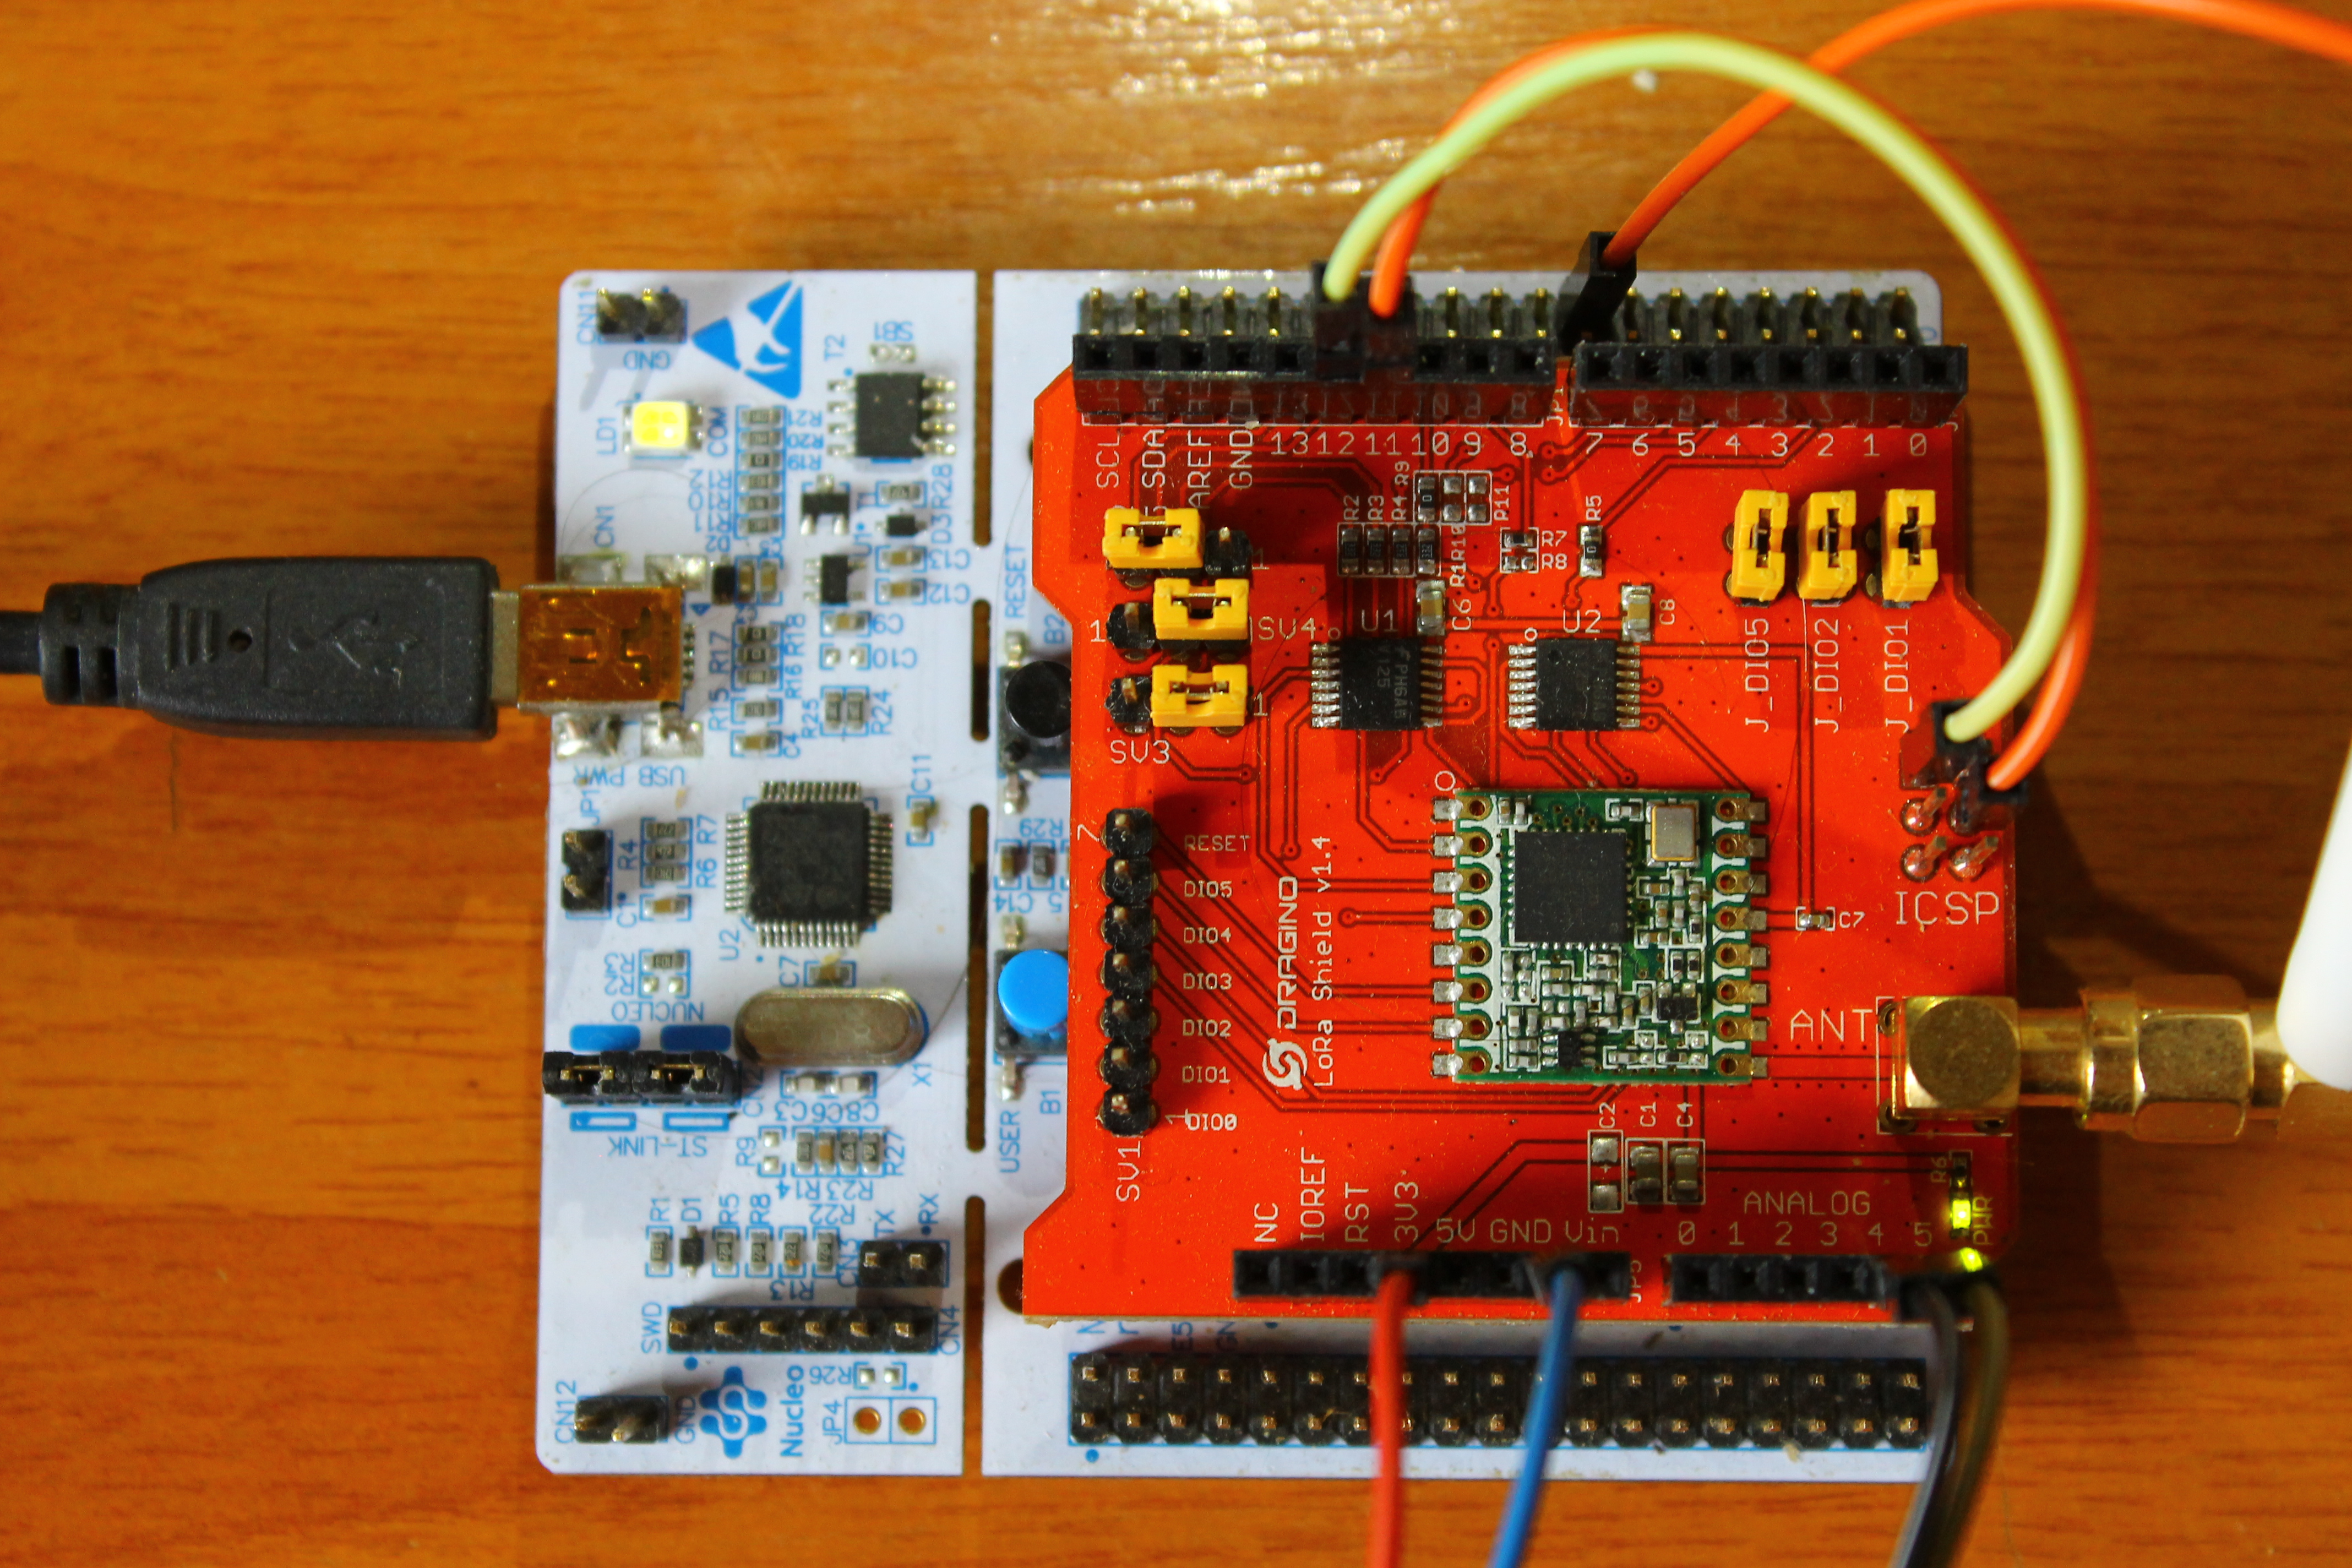
\includegraphics[width=1\textwidth]{foto01}
    \caption{foto zapojení}
    \label{fig:03}
\end{figure}


Pro komunikaci s LoRa transceiverem je tedy použito SPI1, pro komunikaci přes USB je použito USART2 a pro komunikaci přes RS485 je použito UART1.


\begin{table}[h]
    \centering
    \begin{tabular}{ |c|c|c| }
     \hline

     Periférie          & Název pinu & Pin procesoru           \\ \hline \hline
     
                        & RX  &   PC1            \\
    RS485 transceiver   & TX  &   PC0       \\
                        & RTS  &  PB1      \\     \hline

                        & CS    &  PB6             \\
                        & CLK   &  PA5        \\
   LoRa transceiver     & MISO  &  PA6     \\
                        & MOSI  &  PA7        \\
                        & RST   & PC7          \\
                        & DIO0  & PA10         \\
                        \hline

    \end{tabular}
    \caption{Pinout připojení externích periférií k procesoru}
    \label{table:3}
\end{table}


\section{Instalace}
K nahrání zkompilovaného programu do procesoru z PC není potřeba instalovat žádný SW. 
Kit je potřeba připojit k PC přes USB. V PC se to zobrazí jako flash disk. Zkompilovaný program s koncovkou .binary stačí překopírovat na toto zařízení. Po dobu kopírování souboru bliká na kitu LED1 červená/zelená. Jakmile kopírování skončí, program se spustí. Kit je také možné restartovat černým tlačítkem reset.

 Pro uvedení Gatewaye do provozu je nutné se připojit k zařízení přes USB a nastavit všechny parametry viz sekce v tomto dokumentu: "Konfigurace systému".

\newpage
%%%%%%%%%%%%%%%%%%%%%%%%%%%%%%%%%%%%%%%%%%%%%%%%
\section{Zdrojové soubory projektu}
Projekt byl naprogramován v AtolicTrueSTUDIO, což je IDE založené na Eclipse. 
K programování procesoru byly použity standartní HAL knihovny od firmy ST Microelectronics.
Pro šifrování LoRaWAN packetu byla použita knihovna AES-128, dostupná na githubu \cite{AESlib} a knihovna OpenPANA také dostupná z githubu \cite{CMAClib}.
Níže je seznam zdrojových souborů.

\begin{figure}[!h]
    \dirtree{%
        .1 Drivers \DTcomment{STM32 Drivers}.
        .1 Inc\DTcomment{Headers}.
            .2 aes.h\DTcomment{AES-128 library for LoRaWAN packet encryption}.
            .2 cmac.h\DTcomment{library for CMAC calculation in LoRaWAN protocol}.
            .2 LinkedList\_ByteArray.h \DTcomment{Byte array linked list library for stacks}.
            .2 LoRaWAN\_packet.h\DTcomment{LoRaWAN library for packet data decoding}.
            .2 stm32l0xx\_hal\_conf.h\DTcomment{STM32 HAL library}.
            .2 ByteArray.h\DTcomment{Library for Byte array operations}.
            .2 LoRa.h\DTcomment{Library for interfacing LoRa transceiver}.
            .2 main.h\DTcomment{Main file}.
            .2 stm32l0xx\_it.h\DTcomment{STM32 HAL library}.
            .2 eeprom.h\DTcomment{Library for eeprom operations}.
            .2 LoRa\_sensors.h\DTcomment{Library for decoding data from payload}.
            .2 rs485\_protocol.h\DTcomment{Library for RS485 IMA protocol}.
            .2 usb.h \DTcomment{Library for USB communication and system configuration}.
        .1 Src\DTcomment{Sources}.
            .2 aes.c \DTcomment{source file to the aes.h}.
            .2 aes.c \DTcomment{source file to the cmac.h}.
            .2 LinkedList\_ByteArray.c \DTcomment{source file to the LinkedList\_ByteArray.h}.
            .2 LoRaWAN\_packet.c  \DTcomment{source file to the LoRaWAN\_packet.h}.
            .2 stm32l0xx\_hal\_msp.c \DTcomment{HAL source file}.
            .2 ByteArray.c  \DTcomment{source file to the ByteArray.h}.
            .2 LoRa.c \DTcomment{source file to the LoRa.h}.
            .2 main.c \DTcomment{main source file}.
            .2 stm32l0xx\_it.c \DTcomment{HAL source file}.
            .2 eeprom.c \DTcomment{source file to the eeprom.h}.
            .2 LoRa\_sensors.c \DTcomment{source file to the LoRa\_sensors.h}.
            .2 rs485\_protocol.c  \DTcomment{source file to the rs485\_protocol.h}.
            .2 system\_stm32l0xx.c \DTcomment{HAL source file}.
            .2 usb.h \DTcomment{source file to the usb.h}.
    }
\end{figure}



\bibliographystyle{amsalpha}
% \bibliography{0main}	% not used
% \input{references_project1.tex}
\bibliographystyle{csn690}
\bibliography{mybibliographyfile}
\begin{thebibliography}{9}
%%%%%%%%%%%%%%%%%%%%%%%%%%%%%%%%%%%%%%%%%%%%%%%%%%%%%%%%%%%%%%%



% % -------------------------
\bibitem[1]{Design and Implementation of an IoT Assisted Real Time ZigBee Mesh WSN}
H. Ali, W. Y. Chew, F. Khan and S. R. Weller, "Design and implementation of an IoT assisted real-time ZigBee mesh WSN based AMR system for deployment in smart cities," \textit{2017 IEEE International Conference on Smart Energy Grid Engineering (SEGE)}, Oshawa, ON, 2017, pp. 264-270.
[Online]. Available:
\url{
https://ieeexplore.ieee.org/stamp/stamp.jsp?tp=&arnumber=8052810
}
[Accessed: 9-Sep-2019].


% % % -------------------------
\bibitem[2]{Internet of Things (IoT) for building Smart Home System}
T. Malche and P. Maheshwary, "Internet of Things (IoT) for building smart home system," \textit{2017 International Conference on I-SMAC (IoT in Social, Mobile, Analytics and Cloud) (I-SMAC)}, Palladam, 2017, pp. 65-70.
[Online]. Available:
\url{
https://ieeexplore.ieee.org/stamp/stamp.jsp?tp=&arnumber=8058258
}
[Accessed: 9-Sep-2019].


% % -------------------------
\bibitem[3]{A comparative study of LPWAN technologies for large-scale IoTdeployment}
K. Mekki, E. Bajic, F. Chaxel and F. Meyer, "A comparative study of LPWAN technologies for large-scale IoT deployment". \textit{ICT Express}, vol. 5, no. 1, March 2019.
[Online]. Available:
\url{
https://www.sciencedirect.com/science/article/pii/S2405959517302953
}
[Accessed: 9-Sep-2019].

% % -------------------------
\bibitem[4]{Long-Range Communications in Unlicensed Bands}
M. Centenaro, L. Vangelista, A. Zanella and M. Zorzi, "Long-range communications in unlicensed bands: the rising stars in the IoT and smart city scenarios," in \textit{IEEE Wireless Communications}, vol. 23, no. 5, pp. 60-67, October 2016.
[Online]. Available:
\url{
https://ieeexplore.ieee.org/stamp/stamp.jsp?tp=&arnumber=7721743
}
[Accessed: 9-Sep-2019].

% -------------------------
\bibitem[5]{high density LPWAN}
A. Lavric and A. loan Petrariu, "High-Density Low Power Wide Area Networks," \textit{2018 10th International Conference on Electronics, Computers and Artificial Intelligence (ECAI)}, Iasi, Romania, 2018, pp. 1-4.
[Online]. Available:
\url{
https://ieeexplore.ieee.org/stamp/stamp.jsp?tp=&arnumber=8678997
}
[Accessed: 9-Sep-2019].

% % -------------------------
\bibitem[6]{MURS Band for LPWAN Applications}
A. Kosari and D. D. Wentzloff, "MURS Band for LPWAN Applications," \textit{2019 IEEE Topical Conference on Wireless Sensors and Sensor Networks (WiSNet)}, Orlando, FL, USA, 2019, pp. 1-3.
[Online]. Available:
\url{
https://ieeexplore.ieee.org/stamp/stamp.jsp?tp=&arnumber=8711814
}
[Accessed: 9-Sep-2019].


% -------------------------
\bibitem[7]{IoT cisco study}
KRANZ, Maclej. The Internet of Things: 5 Predictions for 2018. CISCO: blog 
[Online]. Available:
\url{
https://blogs.cisco.com/innovation/the-internet-of-things-5-predictions-for-2018
}
[Accessed: 9-Sep-2019].

% % -------------------------
\bibitem[8]{Flexible Wireless Sensor Network for smart lighting applications}
R. F. Fernandes, C. C. Fonseca, D. Brandão, P. Ferrari, A. Flammini and A. Vezzoli, "Flexible Wireless Sensor Network for smart lighting applications," 2014 IEEE International Instrumentation and Measurement Technology Conference (I2MTC) Proceedings, Montevideo, 2014, pp. 434-439.
[Online]. Available:
\url{
https://ieeexplore.ieee.org/stamp/stamp.jsp?tp=&arnumber=6860782
}
[Accessed: 9-Sep-2019].



% % % -------------------------
\bibitem[9]{Building a Smart Home System with WSN and Service Robot}
W. Huiyong, W. Jingyang and H. Min, "Building a Smart Home System with WSN and Service Robot," \textit{2013 Fifth International Conference on Measuring Technology and Mechatronics Automation}, Hong Kong, 2013, pp. 353-356.
[Online]. Available:
\url{
https://ieeexplore.ieee.org/stamp/stamp.jsp?tp=&arnumber=6493740
}
[Accessed: 9-Sep-2019].


% % -------------------------
\bibitem[10]{A Meter Reading System Based on WSN}
Luo Hui, "A meter reading system based on WSN," \textit{2010 International Conference on Optics, Photonics and Energy Engineering (OPEE)}, Wuhan, 2010, pp. 311-314.
[Online]. Available:
\url{
https://ieeexplore.ieee.org/stamp/stamp.jsp?tp=&arnumber=5508121
}
[Accessed: 9-Sep-2019].


% % -------------------------
\bibitem[11]{Smart Water Meter System for User-Centric Consumption Measurement}
M. J. Mudumbe and A. M. Abu-Mahfouz, "Smart water meter system for user-centric consumption measurement," \textit{2015 IEEE 13th International Conference on Industrial Informatics (INDIN)}, Cambridge, 2015, pp. 993-998.
[Online]. Available:
\url{
https://ieeexplore.ieee.org/stamp/stamp.jsp?tp=&arnumber=7281870
}
[Accessed: 9-Sep-2019].


% % -------------------------
\bibitem[12]{Radio Data Infrastructure for Remote Monitoring}
R. K. Kodali, "Radio data infrastructure for remote monitoring system using lora technology," \textit{2017 International Conference on Advances in Computing, Communications and Informatics (ICACCI)}, Udupi, 2017, pp. 467-472.
[Online]. Available:
\url{
https://ieeexplore.ieee.org/stamp/stamp.jsp?tp=&arnumber=8125884
}
[Accessed: 9-Sep-2019].


% % -------------------------
\bibitem[13]{Smart Electric Meter Using LoRA Protocols and Iot applications}
N. Shah and P. S. Sundar, "Smart Electric Meter Using LoRA Protocols and lot applications," \textit{2018 Second International Conference on Electronics, Communication and Aerospace Technology (ICECA)}, Coimbatore, 2018, pp. 1178-1180.
[Online]. Available:
\url{
https://ieeexplore.ieee.org/stamp/stamp.jsp?tp=&arnumber=8474749
}
[Accessed: 9-Sep-2019].



% % -------------------------
\bibitem[14]{ttn}
The Things Network, TODO
[Online]. Available:
\url{
https://www.thethingsnetwork.org/
}
[Accessed: 25-Apr-2020].



% % -------------------------
\bibitem[15]{Implement Smart Farm with IoT Technology}
C. Yoon, M. Huh, S. Kang, J. Park and C. Lee, "Implement smart farm with IoT technology," \textit{2018 20th International Conference on Advanced Communication Technology (ICACT)}, Chuncheon-si Gangwon-do, Korea (South), 2018, pp. 749-752.
[Online]. Available:
\url{
https://ieeexplore.ieee.org/stamp/stamp.jsp?tp=&arnumber=8323908
}
[Accessed: 9-Sep-2019].



% -------------------------
% -------------------------
% -------------------------


% -------------------------
\bibitem[16]{accessControlSystem_eiprocus}
Know about Access Control Systems and Their Types with Features. \textit{Electronics projects focus}
[Online]. Available:
\url{
https://www.elprocus.com/understanding-about-types-of-access-control-systems/
}
[Accessed: 9-Sep-2019].



% -------------------------
% -------------------------
% -------------------------



%___________________
%% notused
\bibitem[17]{iqrf_rf}
\textit{
RF.
}
IQRF Alliance.

[Online]. Available:
\url{
https://www.iqrf.org/technology/rf
}
[Accessed: 9-Jun-2018].



%___________________
%% notused
\bibitem[18]{iqrf_ide}
\textit{
IQRF IDE
}
IQRF Alliance.

[Online]. Available:
\url{
https://www.iqrf.org/technology/iqrf-ide
}
[Accessed: 9-Jun-2018].



%___________________

\bibitem[19]{iqrf_sdk}
\textit{
IQRF SDK.
}
IQRF Alliance.
[Online]. Available:
\url{
https://www.iqrf.org/technology/iqrf-sdk
}
[Accessed: 9-Jun-2018].

%___________________


\bibitem[20]{iqrf_transceivers}
\textit{
Transceivers.
}
IQRF Alliance.

[Online]. Available:
\url{
https://www.iqrf.org/products/transceivers
}
[Accessed: 9-Jun-2018].

%___________________

\bibitem[21]{iqrf_alliance}
\textit{
Three security levels in new IQRF OS 4.0.
}
IQRF Alliance.
[Online]. Available:
\url{
https://www.iqrfalliance.org/news/117-three-security-levels-in-new-iqrf-os-4-0
}
[Accessed: 9-Jun-2018].


\bibitem[22]{paper_iqrf}

[Online]. Available:
\url{
https://ieeexplore.ieee.org/stamp/stamp.jsp?tp=&arnumber=8399666
}
[Accessed: 9-Sep-2019].


%___________________ Wireless M-Bus

\bibitem[23]{EN 13757}
[Online]. Available:
\url{
https://ec.europa.eu/eip/ageing/standards/ict-and-communication/data/en-13757_en
}
[Accessed: 2-Apr-2020].


\bibitem[24]{wirelessMBus_automatizace}
[Online]. Available:
\url{
https://automatizace.hw.cz//sbernice-wireless-mbus-jde-i-bezdratove
}
[Accessed: 9-Jun-2018].

%___________________

\bibitem[25]{wirelessMBus01}
\textit{
Wireless Meter Bus, WM-Bus Technology.
}
Radio-Electronics.
[Online]. Available:
\url{
http://www.radio-electronics.com/info/wireless/wireless-m-bus/basics-tutorial.php
}
[Accessed: 9-Jun-2018].

%___________________

\bibitem[26]{wirelessMBus02}
\textit{
Wireless M-Bus in Industrial Wireless Sensor Networks.
}
Radiocrafts.
[Online]. Available:
\url{
https://radiocrafts.com/technologies/wireless-m-bus-technology-overview/
}
[Accessed: 9-Jun-2018].

%___________________

% page unavailable
% \bibitem[24]{7}
% Radiocrafts: 
% \textit{
% WirelessM-Bus in Industrial Sensor Networks.
% }
% [Online]. Available:
% \url{
% https://radiocrafts.com/uploads/AN024_Using_Wireless_M-BUS_in_Industrial_Sensor_Networks_1_0.pdf
% }
% [Accessed: 9-Jun-2018].

%___________________

\bibitem[27]{wirelessMBus03}
Silicon labs: 
\textit{
WIRELESS M-BUS SOFTWARE IMPLEMENTATION.
}
[Online]. Available:
\url{
https://www.silabs.com/documents/public/application-notes/AN451.pdf
}
[Accessed: 9-Jun-2018].

%___________________

\bibitem[28]{wirelessMBus04}
Compass security:
\textit{
Wireless M-Bus Security Whitepaper Black Hat USA 2013.
}
June 30th. 2013, v1.01.
[Online]. Available:
\url{
https://www.compass-security.com/fileadmin/Datein/Research/Praesentationen/blackhat_2013_wmbus_security_whitepaper.pdf
}
[Accessed: 9-Jun-2018].


% % % -------------------------
% \bibitem[1118]{ZigBee-based Vehicle Access Control System}

% [Online]. Available:
% \url{
% https://ieeexplore.ieee.org/stamp/stamp.jsp?tp=&arnumber=5453569
% }
% [Accessed: 9-Sep-2019].


%___________________

% \bibitem[27]{Zigbee_wiki}
% \textit{
% Zigbee.
% }
% Wikipedia.
% [Online]. Available:
% \url{
% https://en.wikipedia.org/wiki/Zigbee
% }
% [Accessed: 9-Jun-2018].

%___________________


% \bibitem[28]{Zigbee_mit}
% Xueqi Fan, Fransisca Susan, William Long, Shangyan Li: 
% \textit{
% Security Analysis of Zigbee.
% }
% May 18, 2017.
% [Online]. Available:
% \url{
% https://courses.csail.mit.edu/6.857/2017/project/17.pdf
% }
% [Accessed: 9-Jun-2018].

%___________________


\bibitem[29]{Zigbee_alliance_about}
\textit{
The Zigbee Alliance.
}
Zigbee alliance.
[Online]. Available:
\url{
http://www.zigbee.org/zigbee-for-developers/about-us/
}
[Accessed: 9-Jun-2018].

%___________________


\bibitem[30]{Zigbee_alliance_solution}
\textit{
The Zigbee Alliance.
}
Zigbee alliance.
[Online]. Available:
\url{
https://zigbeealliance.org/solution/zigbee/
}
[Accessed: 9-Jun-2018].

%___________________ Bluetooth LE

% \bibitem[30]{13}
% \textit{
% Bluetooth sensor network.
% }
% mikroelektronika.
% [Online]. Available:
% \url{
% https://www.mikroe.com/blog/bluetooth-sensor-network
% }
% [Accessed: 9-Jun-2018].

% %___________________


% \bibitem[31]{14}
% \textit{
% Dispelling Common Bluetooth Misconceptions.
% }
% Sans technology institute.
% [Online]. Available:
% \url{
% https://www.sans.edu/cyber-research/security-laboratory/article/bluetooth
% }
% [Accessed: 9-Jun-2018].

% %___________________


% \bibitem[32]{15}
% \textit{
% Bluetooth radio interface, modulation, \& channels.
% }
% Radioelectronics.
% [Online]. Available:
% \url{
% http://www.radio-electronics.com/info/wireless/bluetooth/radio-interface-modulation.php
% }
% [Accessed: 9-Jun-2018].

% %___________________


% \bibitem[33]{16}
% Kianoosh Karami: 
% \textit{
% BLE Packet.
% } Punch through.  November 07 2016.  
% [Online]. Available:
% \url{
% https://punchthrough.com/blog/posts/maximizing-ble-throughput-part-2-use-larger-att-mtu
% }
% [Accessed: 9-Jun-2018].


\bibitem[31]{BT_alliance}
\textit{
BLE Packet.
}
[Online]. Available:
\url{
https://www.bluetooth.com/learn-about-bluetooth/bluetooth-technology/radio-versions/
}
[Accessed: 9-Jun-2018].


\bibitem[32]{BT_nordic}
\textit{
BLE Packet.
}
[Online]. Available:
\url{
https://blog.nordicsemi.com/getconnected/things-you-should-know-about-bluetooth-range
}
[Accessed: 9-Jun-2018].

%___________________ LoRa



% \bibitem[2217]{17}
% \textit{
% LoRa Wireless for M2M \& IoT.
% }
% Radioelectronics.
% [Online]. Available:
% \url{
% http://www.radio-electronics.com/info/wireless/lora/basics-tutorial.php
% }
% [Accessed: 9-Jun-2018].

% \bibitem[2218]{18}
% \textit{
% LoRa Network: LoRaWAN.
% }
% Radioelectronics.
% [Online]. Available:
% \url{
% http://www.radio-electronics.com/info/wireless/lora/lorawan-network-architecture.php
% }
% [Accessed: 9-Jun-2018].

\bibitem[33]{lorawan_specification}
LoRa Alliance, "LoRaWAN 1.1 Specification", version 1.1, October 11, 2017
[Online]. Available:
\url{
https://lora-alliance.org/sites/default/files/2018-04/lorawantm_specification_-v1.1.pdf
}
[Accessed: 9-Sep-2019].

% \bibitem[32]{lorawan_limits}
% \textit{
% Understanding the Limits of LoRaWAN.
% } IEEE.
% Communications Magazine. January 2017
% [Online]. Available:
% \url{
% https://arxiv.org/pdf/1607.08011.pdf
% }
% [Accessed: 9-Jun-2018].

% \bibitem[2220]{20}
% BRIAN RAY: 
% \textit{
% Use Cases and Considerations for LoRaWAN.
% }
% Link-labs. June 20, 2016.
% [Online]. Available:
% \url{
% https://www.link-labs.com/blog/use-cases-and-considerations-for-lorawan
% }
% [Accessed: 9-Jun-2018].

% \bibitem[2221]{21}
% \textit{
% LoRa Physical Layer \& RF Interface.
% }
% Radioelectronics.
% [Online]. Available:
% \url{
% http://www.radio-electronics.com/info/wireless/lora/rf-interface-physical-layer.php
% }
% [Accessed: 9-Jun-2018].

% \bibitem[2222]{22}
% Kianoosh Karami: 
% \textit{
% BLE Packet
% }
% Punch through. November 07, 2016.
% [Online]. Available:
% \url{
% https://punchthrough.com/blog/posts/maximizing-ble-throughput-part-2-use-larger-att-mtu
% }
% [Accessed: 9-Jun-2018].

% \bibitem[2223]{23}
% \textit{
% Build your own gateway.
% }
% The things network.
% [Online]. Available:
% \url{
% https://www.thethingsnetwork.org/docs/gateways/start/build.html
% }
% [Accessed: 9-Jun-2018].

% \bibitem[2224]{24}
% \textit{
% LoraWAN in Europe.
% }
% Match X.
% [Online]. Available:
% \url{
% https://matchx.io/community/eu/12-lorawan-in-europe
% }
% [Accessed: 9-Jun-2018].

%________________________________________ Z-Wave

% \bibitem[32]{27}
% \textit{
% Z-Wave.
% }
% Z-wawe Alliance.
% [Online]. Available:
% \url{
% http://www.z-wave.com/about
% }
% [Accessed: 9-Jun-2018].


% \bibitem[33]{28}
% \textit{
% Z-Wave.
% }
% Wikipedia.
% [Online]. Available:
% \url{
% https://en.wikipedia.org/wiki/Z-Wave
% }
% [Accessed: 9-Jun-2018].


% %____________________________________________ Sigfox

% \bibitem[2225]{25}
% Ian Poole: 
% \textit{
% SIGFOX for M2M \& IoT.
% }
% Radioelektronics.
% [Online]. Available:
% \url{
% http://www.radio-electronics.com/info/wireless/sigfox/basics-tutorial.php
% }
% [Accessed: 9-Jun-2018].

% \bibitem[2226]{26}
% \textit{
% SIGFOX for white paper security.
% }
% Sigfox. February 2017.
% [Online]. Available:
% \url{
% https://www.sigfox.com/sites/default/files/1701-SIGFOX-White_Paper_Security.pdf
% }
% [Accessed: 9-Jun-2018].


% %__________________________________________________________ Thread

% \bibitem[2229]{29}
% \textit{
% What is thread.
% }
% Thread group.
% [Online]. Available:
% \url{
% https://www.threadgroup.org/What-is-Thread
% }
% [Accessed: 10-Jun-2018].


% \bibitem[2230]{30}
% \textit{
% Thread (network protocol).
% }
% Wikipedia.
% [Online]. Available:
% \url{
% https://en.wikipedia.org/wiki/Thread_(network_protocol)
% }
% [Accessed: 10-Jun-2018].


% \bibitem[2231]{31}
% \textit{
% Experimental Study of Thread
% Mesh Network for Wireless
% Building Automation Systems.
% }
% EXAMENSARBETE INOM ELEKTROTEKNIK. STOCKHOLM. SVERIGE 2016.
% [Online]. Available:
% \url{
% http://www.diva-portal.org/smash/get/diva2:1040491/FULLTEXT02
% }
% [Accessed: 10-Jun-2018].


%__________________________________________________________________________ RPMA


% \bibitem[2232]{32}
% \textit{
% RPMA TECHNOLOGY.
% }
% Internet of things.
% [Online]. Available:
% \url{
% https://theinternetofthings.report/Resources/Whitepapers/4cbc5e5e-6ef8-4455-b8cd-f6e3888624cb_RPMA\%20Technology.pdf
% }
% [Accessed: 10-Jun-2018].

% \bibitem[2233]{rpma_ublox}
% \textit{
% RPMA.
% }
% Ublox.
% [Online]. Available:
% \url{
% https://www.u-blox.com/en/rpma
% }
% [Accessed: 10-Jun-2018].

% \bibitem[2234]{34}
% \textit{
% RPMA TECHNOLOGY.
% }
% Ingenu.
% [Online]. Available:
% \url{
% https://www.ingenu.com/technology/rpma/
% }
% [Accessed: 10-Jun-2018].

% % % -------------------------
\bibitem[34]{Analysis of Propagation Link for Remote Weather}
N. H. Abd Rahman, Y. Yamada, M. H. Husni and N. H. Abdul Aziz, "Analysis of Propagation Link for Remote Weather Monitoring System through LoRa Gateway," \textit{2018 2nd International Conference on Telematics and Future Generation Networks (TAFGEN)}, Kuching, 2018, pp. 55-60.
[Online]. Available:
\url{
https://ieeexplore.ieee.org/stamp/stamp.jsp?tp=&arnumber=8580479
}
[Accessed: 9-Sep-2019].


% % -------------------------
\bibitem[35]{RHF1S001 pdf}
RisingHF, "Outdoor IP64 Temperature and Humidity LoRaWAN sensor RHF1S001", version 1.2, 2015
[Online]. Available:
\url{
http://www.objenious.com/wp-content/uploads/2016/10/RHF-DS01588Outdoor-IP64-Tempratrure-and-Humidity-LoRaWAN-Sensor-RHF1S001_V1.3.pdf
}
[Accessed: 9-Sep-2019].

% % -------------------------
\bibitem[36]{lwSecur}
Robert Miller.
\textit{
LoRa Security
Building a Secure LoRa Solution.
}
MWR Labs Whitepaper.
[Online]. Available:
\url{
https://labs.mwrinfosecurity.com/assets/BlogFiles/mwri-LoRa-security-guide-1.2-2016-03-22.pdf
}
[Accessed: 20-Sep-2019].



% % -------------------------

\bibitem[37]{nucleo-l073RZ_ST}
\textit{
NUCLEO-L073RZ.
}
ST Microelectronics
[Online]. Available:
\url{
https://www.st.com/en/evaluation-tools/nucleo-l073rz.html
}
[Accessed: 20-Sep-2019].


%___________________

\bibitem[38]{RFM95w}
\textit{
RFM95/96/97/98(W) - Low Power Long Range Transceiver Module}.
HopeRF electronic.
V1.0.
[Online]. Available:
\url{
https://www.hoperf.com/modules/lora/RFM95.html
}
[Accessed: 20-Sep-2019].

%___________________


\bibitem[39]{draginoWiki}
\textit{
Lora Shield.
}
Dragino.
[Online]. Available:
\url{
http://wiki.dragino.com/index.php?title=Lora_Shield
}
[Accessed: 20-Sep-2019].

%___________________


\bibitem[40]{rs485tr}
\textit{
SparkFun Transceiver Breakout - RS-485
}
Sparkfun.
[Online]. Available:
\url{
https://www.sparkfun.com/products/10124
}
[Accessed: 20-Sep-2019].


%___________________

\bibitem[41]{nucleo-l073RZ_Mbed}
\textit{
NUCLEO-L073RZ
}
ARM Mbed.
[Online]. Available:
\url{
https://os.mbed.com/platforms/ST-Nucleo-L073RZ/
}
[Accessed: 20-Sep-2019].

%___________________

\bibitem[42]{stm32cubemx}

[Online]. Available:
\url{
https://www.st.com/en/development-tools/stm32cubemx.html
}
[Accessed: 20-Sep-2019].

%___________________

\bibitem[43]{vscode}

[Online]. Available:
\url{
https://code.visualstudio.com/
}
[Accessed: 20-Sep-2020].

%___________________

\bibitem[44]{arm-none-eabi-gcc}

[Online]. Available:
\url{
https://developer.arm.com/tools-and-software/open-source-software/developer-tools/gnu-toolchain/gnu-rm/downloads
}
[Accessed: 20-Sep-2020].

%___________________

\bibitem[45]{makefile}

[Online]. Available:
\url{
https://www.gnu.org/software/make/manual/make.html
}
[Accessed: 20-Sep-2019].

%___________________

\bibitem[46]{st-flash}

[Online]. Available:
\url{
https://github.com/texane/stlink
}
[Accessed: 20-Sep-2019].

%___________________

\bibitem[47]{cortex-debug}

[Online]. Available:
\url{
https://marketplace.visualstudio.com/items?itemName=marus25.cortex-debug
}
[Accessed: 20-Sep-2019].



%___________________        used libraries


\bibitem[48]{lib_tiny-AES128-C}
\textit{
tiny-AES128-C
}
bitdust.
[Online]. Available:
\url{
https://github.com/bitdust/tiny-AES128-C
}
[Accessed: 20-Sep-2019].

%___________________


\bibitem[49]{lib_openpana}
\textit{
openpana.
}
OpenPANA.
[Online]. Available:
\url{
https://github.com/OpenPANA/openpana
}
[Accessed: 20-Sep-2019].

%___________________


\bibitem[50]{nucleo-l432KC_ST}
\textit{
NUCLEO-L432KC.
}
ST Microelectronics
[Online]. Available:
\url{
https://www.st.com/en/microcontrollers-microprocessors/stm32l432kc.html
}
[Accessed: 25-Apr-2020].




















% -------------------------
% -------------------------
% -------------------------





% % % % -------------------------
% \bibitem[16]{LoRaWAN Evaluation for IoT Communications}
% D. Singh, O. G. Aliu and M. Kretschmer, "LoRa WanEvaluation for IoT Communications," \textit{2018 International Conference on Advances in Computing, Communications and Informatics (ICACCI)}, Bangalore, 2018, pp. 163-171.
% [Online]. Available:
% \url{
% https://ieeexplore.ieee.org/stamp/stamp.jsp?tp=&arnumber=8554713
% }
% [Accessed: 9-Sep-2019].

% % % -------------------------
% \bibitem[18]{Internet of Things (IoT) using LoRa technology}
% A. Zourmand, A. L. Kun Hing, C. Wai Hung and M. AbdulRehman, "Internet of Things (IoT) using LoRa technology," \textit{2019 IEEE International Conference on Automatic Control and Intelligent Systems (I2CACIS)}, Selangor, Malaysia, 2019, pp. 324-330.
% [Online]. Available:
% \url{
% https://ieeexplore.ieee.org/stamp/stamp.jsp?tp=&arnumber=8825008
% }
% [Accessed: 9-Sep-2019].













% % % -------------------------
% \bibitem[]{}

% [Online]. Available:
% \url{

% }
% [Accessed: 9-Sep-2019].


% % % -------------------------
% \bibitem[]{}

% [Online]. Available:
% \url{

% }
% [Accessed: 9-Sep-2019].


% % % -------------------------
% \bibitem[]{}

% [Online]. Available:
% \url{

% }
% [Accessed: 9-Sep-2019].





\end{thebibliography}

%\appendix


\end{document}